\section{Datataking Strategy}
%In Run~I the rate of collisions was 15 MHz, which will double in Run~II. The
%output rate of events stored on tape will change from 5 kHz in Run~I to 12.5 KHz
%in Run~II.
% The
% output rate of L0 is fixed to 1MHz by the front end electronics used to read out
% the detector. 
%In Run~I the event reconstruction performed online by the trigger was simpler and
%quicker than the one performed offline on triggered events in order to meet time
%contraints; the final detector calibration and an improved alignment were obtained
%offline on triggered data and the data used for most of the physics results was
%processed at the end of the year using the latest constants.

A schematic diagram showing the trigger data flow in Run 2 is depicted
in Figure~\ref{fig:trigger}.  The maximum rate at which events can be
read out of the detector is imposed by the front-end electronics and
corresponds to a rate of 1.1\,MHz. In order to determine which events
are kept, hardware triggers based on field-programmable gate arrays
are used with a fixed latency of $4\,\mu {\rm s}$. Information from
the \ecal, \hcal, and muon stations is used in separate \lz
triggers. Events selected by \lz are transferred to the High Level
Trigger (\hlt) for further analysis and selection.

\begin{figure}[h]
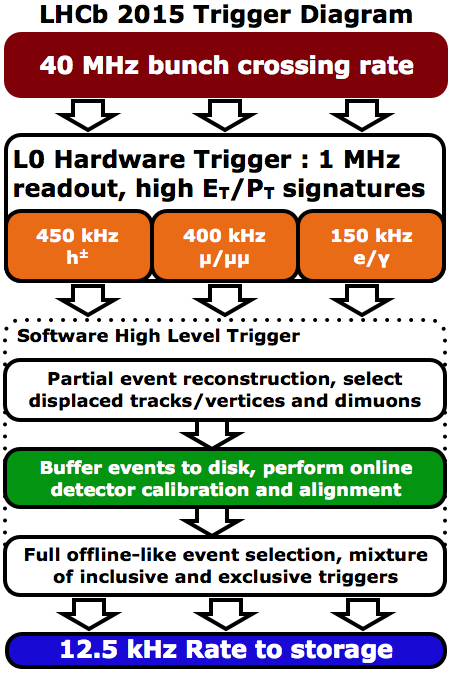
\includegraphics[width=14pc]{../figures/trigger.png}\hspace{2pc}%
\begin{minipage}[b]{14pc}\caption{\label{fig:trigger}Trigger strategy for Run~II: after the hardware stage and a first software stage based on a partial
    reconstruction, the selected events are buffered on disk while the
    real-time calibration and alignment are performed. The second
    stage of the software trigger performs the same reconstruction
    performed offline using the same calibration and alignment.}
\end{minipage}
\end{figure}

%In Run~II this deferral strategy is exploited even further as shown in Figure
%\ref{fig:trigger}; after L0 and \hltone all the selected events are buffered on
%disk allowing to have more time to process a single event (150 ms/event in
%Run~I, 350 ms/event in Run~II).  The automatic calibration and alignment is
%performed in the trigger farm within a few minutes.  The same offline
%reconstruction is run in \hlttwo thanks to this larger time budget together with
%the reduced time requested by the improved track reconstruction.


% In Run~II the LHCb trigger strategy is different as shown in Figure \ref{fig:trigger}.
% After the hardware stage, and a first software stage (\hltone) based on a partial
% reconstruction, the selected events are buffered on disk while the
% automatic calibration and alignment is performed in a few
% minutes in the trigger farm.
% The second stage of the
% software trigger (\hlttwo) performs the same reconstruction run
% offline by using the same calibration and alignment.

The \hlt is divided into two stages, \hltone and \hlttwo, processed on
an Event Filter Farm (EFF) of approximately 1700 nodes with 27000
physical cores,   which allows to simultaneosuly run 50000 processes
using hyper-threading technology.  Events selected by an \hltone
trigger are buffered to the local harddisk of each node before being
processed by \hlttwo.  This buffering is done for two purposes :
events can be processed during inter-fill periods, and the detector
can be calibrated and aligned run-by-run before the \hlttwo stage.
During 2012 LHC spent only approximately $30\%$ of its time in stable
running due to e.g.  planned technical stops, machine developement
phases and the time between data taking fills needed for the ramping
of the LHC dipole magnets.  The usage of the local disks, around
5~PBytes in total, allows around 150~hours of LHC datataking to be
buffered, and has enabled \lhcb to fully utilize the EFF throughout
the tecnical stops and machine development phases (with the exception
of the annual winter shutdown of the LHC), more than doubling the
effective available processing power.  It is this buffering which
allows the full offline event reconstruction to be executed in the
\hlttwo stage.

The \hltone trigger performs an inclusive selection of  events based
on one or two track combinations, the presence of muon tracks
displaced from the primary vertex, or dimuon combinations in the
event. Crucially, it is also able to select the types of events
required by each alignment and calibration task, and these events are
flagged by specific routing bits which allow them to be streamed to
the relevant tasks. There are two kinds of alignment and calibration
tasks : those which are expected to change for each run, and those
which are expected to change less frequently, perhaps once per fill or
once every few fills. In the first case, which mainly concerns the
calibration of the RICH detectors, the calibration constants are
calculated for each run and updated before the \hlttwo processing of
that run. In the second case, the alignment and calibration constants
are calculated for each run, and an automated monitoring task checks
if they have changed by more than a certain threshold with respect to
the previous values. When such a significant variation is observed, a
change of run is triggered. The new constants are updated for the new
run to be used online by the two stages of the software trigger, and
offline, for every further reconstruction and selection. As these
variations are infrequent and slow, the events collected in the run
preceeding this update are still reconstructed in \hlttwo and offline
with the same constants used by \hltone.  Once the detector is fully
aligned and calibrated the events are processed by \hlttwo, where a
full event reconstruction is performed. 

%As exception the RICH calibration
%constants are updated for each run after \hltone both online, in \hlttwo, and offline
%as the previous trigger stages do not rely on hadron identification
%requirements.

% This part should be moved to the introduction
This strategy has several advantages: firstly it minimises the
difference between the online and offline performance, allowing a more
effective trigger selection that can take advantage of the hadron
identification information. For example charm physics is limited by
trigger output rate contraints; using hadron identification in the
trigger allows to have a higher selection efficiency and purity for
the doubly Cabibbo suppressed modes and, at the same time, satisfy the
output rate constraints by pre-scaling the more abundant Cabibbo
favourite modes.  Secondly it ensures the stability of the alignment
quality and hence of the physics performance.  Finally, as in Run~II
the last level of the trigger performs the same reconstruction as the
one performed offline,
% \cite{Barbara}
it will be possible to run some physics analyses, with the same
offline performance, directly on the output of the trigger using the
special stream of data known as Turbo stream \cite{Sean}. This
approach has the advantage that, for some events, it will be possible
to save only the information on the signal candidate tracks ($\sim$ 5
kB per event) instead of all the electronic signals recorded from the
detector ($\sim$ 70 kB per event). This decrease of more than one
order of magnitude of the event size will allow a higher selection
rate, for example in the charm analyses that during Run~I used trigger
lines which were pre-scaled due to output rate requirements. It is
obvious that the real-time alignment and calibration becomes essential
when the raw event is not saved.

